\chapter {IMPLEMENTASI}

\section{Lingkungan Implementasi}

Lingkungan implementasi dan pengembangan menggunakan sebuah komputer dengan spesifikasi perangkat lunak dan perangkat keras sebagai berikut.

\begin{enumerate}
	\item Perangkat Keras
	\par Implementasi tugas akhir ini menggunakan desktop personal computer ASUS X555Q. Namun digunakan untuk menjalankan Google Colab dengan spesifikasi :
	\begin{enumerate}
		\item GPU: 1x Tesla K80 , having 2496 CUDA cores, compute 3.7, 12GB(11.439GB Usable) GDDR5 VRAM
		\item CPU: 1x single core hyper threaded i.e(1 core, 2 threads) Xeon Processors @2.3Ghz (No Turbo Boost) , 45 MB Cache
	\end{enumerate}
	\item Perangkat Lunak
	\begin{enumerate}
		\item Sistem Operasi Linux 18.04 64-bit
		\item Android Studio
		\item Bahasa Pemrograman Java
		\item Bahasa Pemrograman Python
		\item Library Keras
	\end{enumerate}
\end{enumerate}


\section{Implementasi Ekstraksi Fitur}
Subbab ini menjabarkan implementasi ekstraksi fitur, yang akan dijelaskan pada pseudocode dibawah. Hal-hal yang perlu dilakukan pada ekstraksi fitur adalah membaca semua gambar, membuka arsitektur yang dipilih, melakukan preprocess pada gambar, dan menyimpan fitur-fitur dari gambar yang telah diprediksi dengan model.
\begin{lstlisting}[language=python, caption=Pseudocode implementasi ekstraksi fitur, label=code:read_h5, firstnumber=1]
train_path = os.listdir(path)
labels = []
for folder in train_path.size
	labels += folder
	
model = load_architecture()
features = []

for i, label in train_path
	image = load_image()
	image = preprocess_input(image)
	feature = model.predict(image)
	features += feature.flatten()
dump_model()
\end{lstlisting}

\section{Implementasi Pelatihan}
\par Berikut adalah implementasi sumber kode untuk melakukan pelatihan dari data yang sudah diekstraksi. Pada tahap ini kita perlu membuka data dari gambar yang telah diekstrak sebelumnya dan mencocokkannya dengan algoritma Logistic Regression. 
\par Setelah itu dari model yang telah dibuat, dilakukan prediksi pada tiap gambar dari data test untuk mengevaluasi seberapa bagus model tersebut. Jika sudah selesai, model akan disimpan ke dalam file berekstensi \textit{pickle}. File \textit{pickle} inilah yang nanti akan dipakai untuk mengklasifikasi daun pada data sebenarnya.
\begin{lstlisting}[language=python, caption=Pseudocode implementasi ekstraksi fitur, label=code:read_h5, firstnumber=1]
data = load_features()
label = load_label()

test_path = os.listdir(path)
test_label = []
test_data = []
for folder in test_path.size
	labels += folder
	test_data += extract_images(folder)
	
model = LogisticRegression()
model.fit(data, label)

for label, features in test_label, test_data
	prediction = model.predict(features)
	if label == prediction
		accuracy +=1

\end{lstlisting}

\section{Implementasi Aplikasi Android}
\par Implementasi pada Android terdiri dari tiga kelas, yaitu kelas MainActivity, kelas UploadActivity dan kelas PredictActivity. Masing-masing kelas pada aplikasi akan terhubung dengan satu view berekstensi xml.

\par Aplikasi ini dapat dijalankan oleh perangkat Android 5.0 keatas. Untuk menjalankan fungsi Predict dan Upload, pengguna harus memastikan telah memberi izin pada aplikasi untuk mengakses kamera. Pada semua fungsi, izin untuk akses internet dibutuhkan karena semua fungsi memerlukan koneksi untuk terhubung ke server.
Berikut adalah implementasi dari aplikasi Android. 
\subsection{Implementasi Kelas MainActivity}
\par Pada kelas MainActivity akan dipanggil file \textbf{activity\_main.xml} yang akan menghasilkan tampilan pada laman pertama di aplikasi. Pada kelas MainActivity juga semua \textit{permission} yang dibutuhkan untuk menjalankan aplikasi akan dicek, yaitu \textit{permission} akses ke kamera dan internet. Apabila \textit{permission} belum diberikan maka aplikasi akan meminta \textit{permission} untuk mengakses kamera dan internet. Tampilan yang muncul adalah seperti ini.
\begin{figure}[H]
	\centering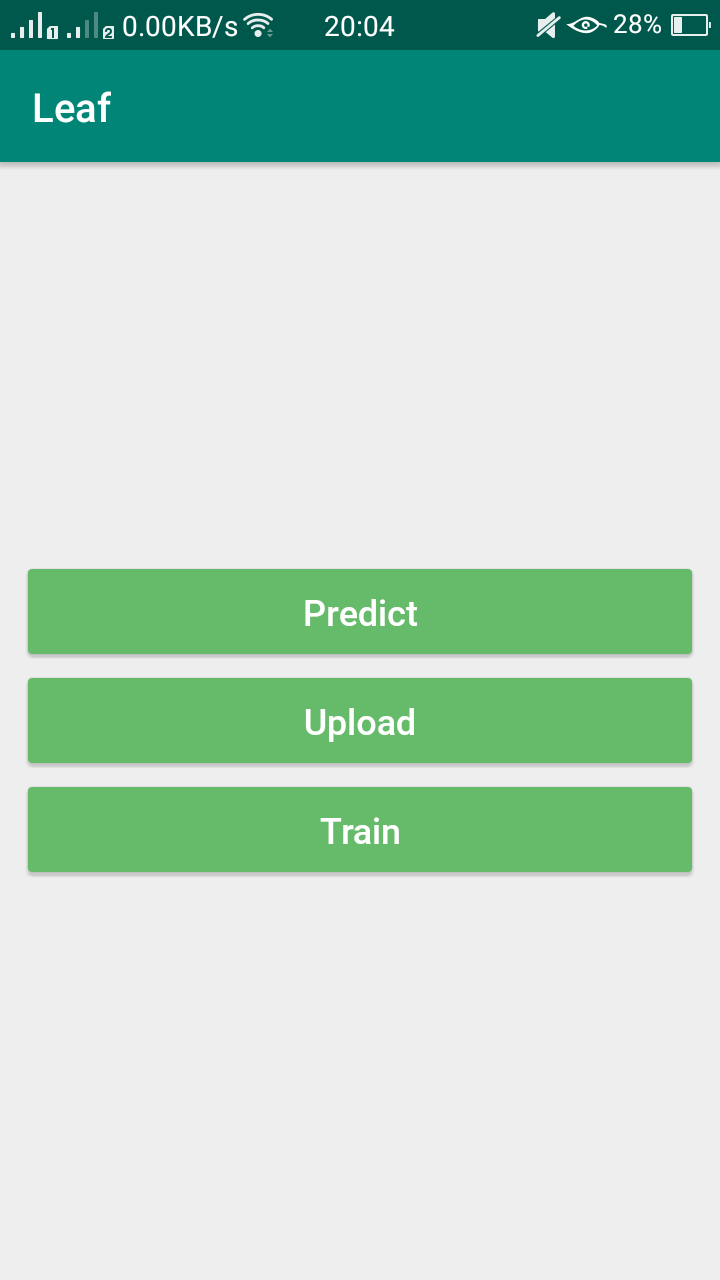
\includegraphics[width=0.6\textwidth]{bab4/figures/main.png}
	\caption{Tampilan awal}
	\label{fig:main}
\end{figure}

\subsection{Implementasi Kelas UploadActivity}
\par Pada kelas UploadActivity pengguna dapat mengunggah gambar beberapa kali dengan nama daun tertentu. Dengan adanya unggahan dari pengguna maka dataset akan bertambah.

\par Fitur Upload menggunakan library \textit{fotoapparat} untuk membuka kamera pada ponsel. Gambar yang ditangkap akan diubah dalam bentuk string sebelum dikirim ke server. Untuk mengirim data ke server digunakan library Retrofit2.

\par Berikut adalah tampilan dari laman upload.
\begin{figure}[H]
	\centering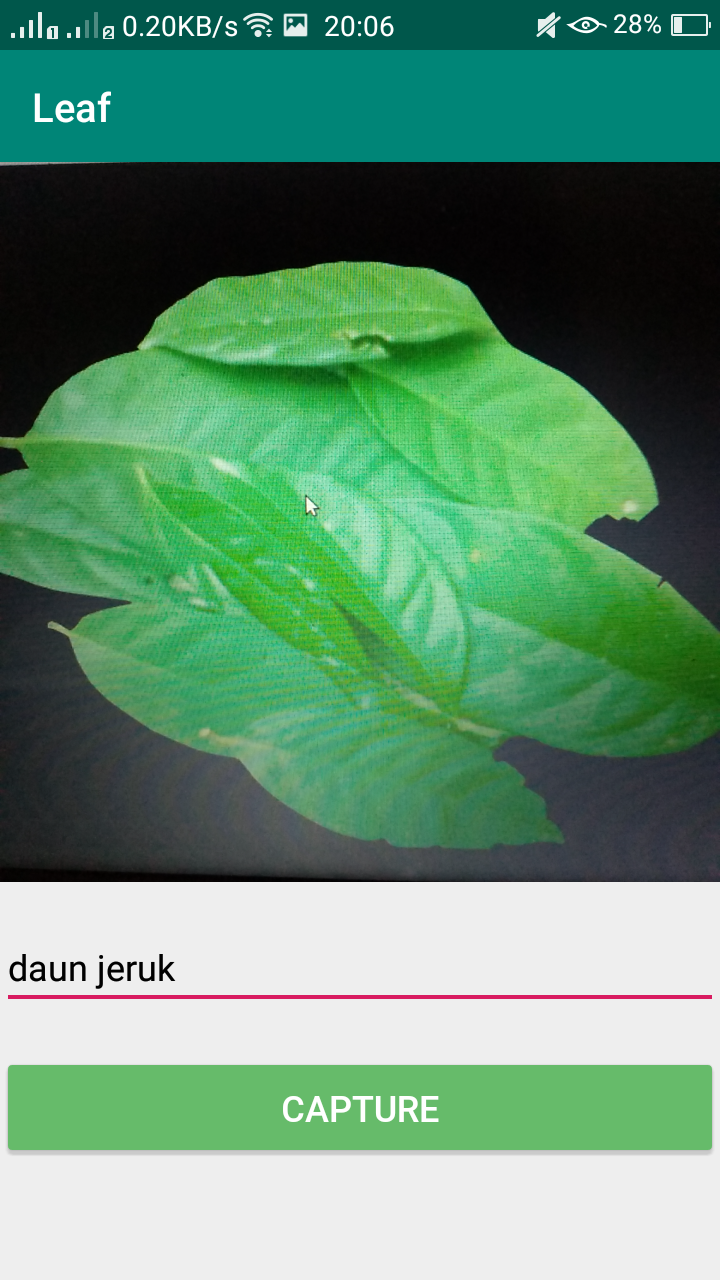
\includegraphics[width=0.6\textwidth]{bab4/figures/upload.png}
	\caption{Tampilan Upload}
	\label{fig:upload}
\end{figure}

\subsection{Implementasi Kelas PredictActivity}

\par Kelas PredictActivity mirip seperti kelas UploadActivity dalam hal tampilan, bedanya adalah kelas ini ketika menembak API pada server akan mendapatkan response berupa nama daun yang diprediksi. Tampilan dari fitur Predict adalah sebagai berikut.
\begin{figure}[H]
	\centering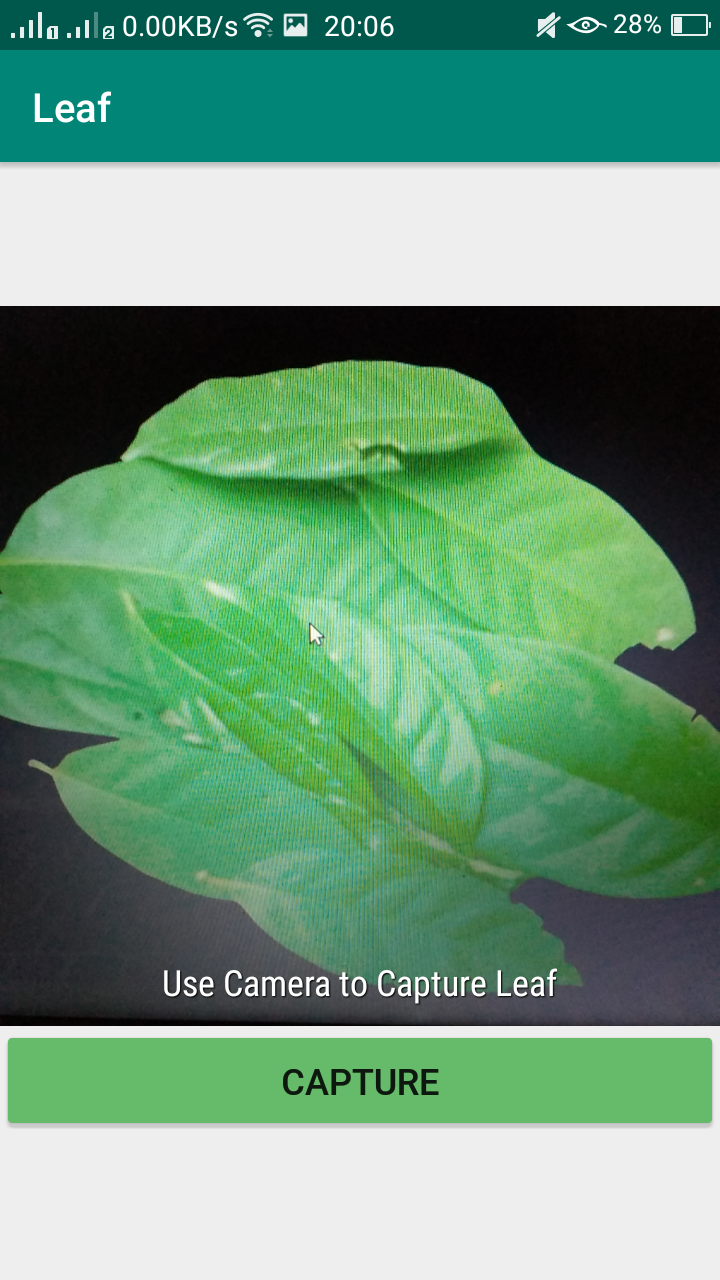
\includegraphics[width=0.7\textwidth]{bab4/figures/predict.png}
	\caption{Tampilan Predict}
	\label{fig:predict}
\end{figure}
\subsection{API}
\par Berikut adalah sumber kode untuk memanggil API pada server.

\begin{lstlisting}[language=python, caption=Pemanggilan API menggunakan Retrofit2, label=code:api, firstnumber=0]
public interface ApiClientAttendance {
@FormUrlEncoded
@POST("/upload/")
Call<ResponseApi> upload(@Field("name") String name,
@Field("image") String image);

@POST("/train/")
Call<ResponseApi> train();

@FormUrlEncoded
@POST("/predict/")
Call<ResponseApi> predict(@Field("image") String image);
}
\end{lstlisting}

\section{Implementasi Backend}
Untuk implementasi backend, yang dibutuhkan adalah \textit{Controller} saja. \textit{Controller} ini yang akan menerima request dan menjalankan program serta mengirim response.
Sumber kode untuk implementasi backend terlampir.